\documentclass[a4paper,12pt]{kth-mag}
\usepackage[T1]{fontenc}
\usepackage{textcomp}
\usepackage{lmodern}
\usepackage[utf8]{inputenc}
\usepackage[swedish,english]{babel}
\usepackage{modifications}
\usepackage{booktabs}
\usepackage{amsmath}
\usepackage{graphicx}
% package for bibliography
\usepackage{natbib}

\setcounter{secnumdepth}{4}
\setcounter{tocdepth}{4}

\title{Lorem ipsum dolor sit amet, sed diam nonummy nibh eui
       mod tincidunt ut laoreet dol}

\subtitle{Duis autem vel eum iruire dolor in hendrerit in
          vulputate velit esse molestie consequat, vel illum
          dolore eu feugiat null}
\foreigntitle{Titel på rapporten på svenska}

\author{Angelina von Gegerfelt\\Kashmir Klingestedt}
\date{\today}
\selectlanguage{swedish}
\blurb{Degree Project in Computer Science, DD143X\\Supervisor: Arvind Kumar\\Examiner: Örjan Ekeberg}
\trita{Stockholm, Sweden \today}

\begin{document}

\frontmatter
\pagestyle{empty}
\removepagenumbers
\maketitle
\selectlanguage{english}

\begin{abstract}
Today an increasing amount of systems make use of Natural Language Interfaces (NLIs), which make them easy and efficient to use. The purpose of this research was to gain an increased understanding of the usability of different input methods for NLIs. This was done by implementing two versions of a text-based game with an NLI, where one version used speech as input method and the other used text. Tests were then performed with 9 test users that all played through both versions of the game and then evaluated them individually using the System Usability Scale. It was found that text was better as input method on all aspects. Speech however scored high when the users felt confident in their English competence, acknowledging the possibility of using speech as input method for NLIs.
 %includes the english abstract
\end{abstract}

\begin{foreignabstract}{swedish}
Idag använder en ökande mängd system naturliga språkgränssnitt, vilket gör dem enkla och effektiva att använda. Syftet med denna forskning var att få en ökad förståelse för användbarheten av olika inmatningsmetoder för naturliga språkgränssnitt. Detta gjordes genom att skapa två versioner av ett text-baserat spel med ett naturligt språkgränssnitt, där en version använde tal som inmatningsmetod och andra använde text. Tester utfördes sedan med användare som alla spelade igenom båda versionerna av spelet och sedan utvärderade dem individuellt med hjälp av System Usability Scale, ett system för att mäta graden av användbarhet. Det konstaterades att text fungerade bättre som inmatningsmetod ur alla aspekter. Tal fick dock en hög poäng när användarna kände sig säkra på sin engelska kompetens, vilket talar för möjligheten att använda tal som en inmatningsmetod för naturliga gränssnitt. %includes the swedish abstract
\end{foreignabstract}
\newpage

\tableofcontents*
\mainmatter
\pagestyle{newchap}

\chapter{Introduction}
A system that has a Natural Language Interface (NLI) enables the user to interact with the system using natural language, which is a language that has developed as a method of communicating between people \citep{NatLan}. The input methods may vary, where some examples are speech, text and body language. A system like this is practical since the user does not have to learn a new interaction technique, such as a programming language or hotkeys, in order to use the system effectively.

Development of natural language as an input method for interacting with systems has been an ongoing process since the late 1940s. At that time the work was focused on machine translation with goals such as translating text or speech from one language to another \citep{Jones}. Today implementations of NLIs are highly encouraged and many frequently used systems include it, such as Google Search and Apple's Siri. Many systems with NLIs are open source, meaning anyone can make use of and contribute to the development of even better NLIs.

The research presented in this paper aims to evaluate and compare two different natural language input methods, namely text and speech. This is done by the use of gamification, where the game is inspired by existing text-based adventure games. The evaluation is based on the ISO-definition of usability, which focuses on the effectiveness, efficiency and satisfaction of a product. \citep{ISO} This is because the ISO-defenitions are created by experts representing 161 countries and are globally accepted as standard.

\section{Problem Statement}
Comparing the two natural language input methods text and speech, which one has the highest usability level according to the ISO-definition of usability?

\section{Scope}
The area of natural languages include additional types of communication other than text and speech, such as body language and touch, although in this research the focus is solely on text and speech. The grammatical strictness of the input differs between different NLIs. In this research a moderately grammatically strict NLI is used for both text and speech, where the input must include a verb and a noun so that the system can comprehend it.

\section{Purpose}
This research has been done in order to increase the understanding of the usability of text and speech input when it comes to Natural Language Interfaces. This knowledge is meant to contribute to the future development of NLIs with text or speech as input methods, in matters such as which input method to use and the effects of using either method.

%\section{Disposition}

\section{Terminology}

\begin{table}[ht]
  \centering
  \begin{tabular}{ccc}
    \toprule
    Expression & Abbrevation & Deffinition\\
    \midrule
    Gamification & - & The application of typical\\
    & & elements of game playing\\
    & & to other areas of activity \\
    \\
    Natural Language & NLI & A way for the user to\\
    Interface & & interact with a system or\\ 
    & & program by the use of\\
    & & human natural language\\
    \\
    Natural Language & NLP & Derives meaning from natural\\
    Processing & & language input and converts\\
    & & it into something the computer\\
    & & can understand and vice versa\\
    \\
    System Usability & SUS & System to measure level of\\
    Scale & &  usability\\
    \bottomrule
  \end{tabular}
  \caption{Short definitions of relevant expressions}\label{termin}
\end{table}

\chapter{Background}
\section{Natural Language}
A natural language is any language that develops naturally in humans through use and repetition without any conscious planning or premeditation of their own. These are the languages human beings use to communicate with each other, whether by speech, signing, touch or writing. They are distinguished from constructed and formal languages such as those used to program computers or to study logic.
 
\subsection{Natural Language Interface}
A Natural Language Interface (NLI) is a way for the user to interact with a system or program in a more natural and intuitive way. NLI have many advantages over other systems, such as that it is flexible, people need little training to use it and it can be allowed to do multiple things at once due to uses of pronouns, quantification and context. In general , NLI’s primary function is that they support and deal with the user’s view of the system and translates it into those actually used by the system \citep{Hend}. A few examples of working consumer NLI are Wolfram Alpha, Siri and Google Search.

\subsection{Natural Language Processing}
Natural Language Processing (NLP) explores how computers can be used to understand and manipulate natural language \citep{Gobi}. The input might be text, speech or other. NLP can be used for translation into another language, to comprehend and represent the content of text, to build/search a database or to maintain a dialogue with a user as part of an interface for database/information retrieval. \citep{Allen} NLP can be seen as a backend to an NLI.

\section{Speech Recognition}
Speech Recognition (SR) systems have been researched and developed as a worldwide activity because of the potential this brings for applications, such as to have voice-interactive management, voice dictation and spoken language translation. Although many successes has been had in the development of practical and useful SR systems, there are still limitations to what can be done. The speech signal is one of the most complex signals that humans try to work with. There is also the fact that human’s vocal systems differ between humans and things can be said in different ways. However, various SR systems have been integrated into consumer-technology today (Siri and Google Now, for example), so we are still making advances with the technology. \citep{SR}

\section{Zork and Text-Based Adventure Games}
%USE A SOURCE
The first version of Zork was written in 1977–1979 and it is one of the earliest interactive fiction computer games. Zork distinguished itself in its genre as an especially rich game, in terms of both the quality of the storytelling and the sophistication of its text parser, which was not limited to simple verb-noun commands (e.g. ``hit troll''), but recognized some prepositions and conjunctions (e.g. ``hit the troll with the Elvish sword''). \citep{Zork}

\section{Previous Research}

\chapter{Method}
\section{The Game}
The game is inspired by the previously mentioned Zork. It consists of a few rooms and tasks to be performed before reaching a victory scenario. The game differs in environments and plot between the different implementations of NLIs, which requires the user to input different commands in order to win. One version uses typing to control your character’s actions and the other uses speech. The reason we decided to create two implementations is so that a user who has played one control-scheme could still play the other without having the benefit of knowing what is required to win.

\subsection{Plot}
The user play as a bunny that has escaped its cage and is on the hunt for food. They need to eat three crackers in each game in order to ease their hunger and win the game. In the speech version the user is a house-pet and is in an apartment and has the ability to be in the kitchen, the livingroom and the bedroom. In the text version they are a class-pet in a school and can visit the classroom, the hallway and the cafeteria.

\section{Implementation}
When implementing the different versions of the game existing open source libraries were used for word tagging and speech recognition, which were then linked to our own built parser. The parser takes two words as arguments: one verb and one noun. These words are sorted out from the user's command line using the word tagger. The parser then generates the proper response by first handling the verb and then linking the action to the given noun. Verbs handled in the parser are ``go'', ``look'', ``take'', ``eat'' and ``use''. Several synonyms to these verbs are also handled by first sending them through a synonym checker that converts them to one of the five verbs handled by the parser. If the verb is not recognized the game responds with ``Try something else''.

\subsection{Programming Language}
The choice of programming language depended on which existing libraries to be used in the game. It turned out that Java was convenient to use since both of us were comfortable using it and there were many libraries to choose from that were adjusted to work in Java.

By using the already existing libraries our own code needed a lot of dependencies. Therefore the development of the game was done in an integrated development environment (IDE) called Eclipse, which provide a lot of handy tools whereof some for easily handling dependencies. To synchronize our coding progress with each other Git was used, which is a source code management system.

\subsection{Stanford POSTagger}
The library which was used for tagging command words is the Stanford Part-Of-Speech Tagger. It is part of the Stanford CoreNLP, which is a suite of core NLP tools. A Part-Of-Speech Tagger (POS Tagger) is a piece of software that reads text in some language and assigns parts of speech to each word, such as noun, verb, adjective, etc. \citep{POSTagger}

By tagging each word in the user's command line it was possible to sort out which command words were verbs and nouns, the types handled in the parser. By doing this the user was able to communicate with the game using natural language. For example commands like ``take the toy located under the couch in the livingroom'' will be handled as ``take toy'', since those words are the verb and noun in the command. Some commands run through the Stanford POSTagger will however be tagged incorrectly if proper grammar is not used. For example when using the command ``use key on door'' the word ``use'' gets tagged as a noun instead of a verb, however if you instead use the command ``use the key on the door'' the word ``use'' gets tagged as a verb. To handle this issue all nouns were run through the synonym checker as well to see if it matched any of our verbs.

\subsection{Sphinx4}
The Sphinx4 speech recognition system is the latest addition to Carnegie Mellon University's repository of the Sphinx speech recognition systems. It is universal in its acceptance of various kinds of grammars and language models, types of acoustic models and feature streams. Sphinx 4 is developed entirely in the Java programming language and is widely used, which made it suitable for use in the game. \citep{Sphinx4}

Sphinx4 is used solely in the speech version of the game, where the user give commands through speech using a microphone. When a command is spoken, Sphinx4 recognizes the separate words and then converts the command to text. It is then sent to the Stanford POSTagger, etc.

Which words and command structures Sphinx4 can recognize is specified in grammar files (with extension .gram). For example specific verbs and nouns can be specified and then the command structure can be set as <verb> <noun>, which would make Sphinx4 recognize commands like ``use key'' but not commands like ``use the small golden key''. In the game the speech command structure is set as

<command> = <verb> <conjunction> <determiner> <noun> | <cmd>.

The straight line symbolizes ``or'', so either structure separated by the straight line is acceptable. The conjunctions and determiners are optional, making both commands like ``go to the livingroom'' and ``go livingroom'' recognizable. The <cmd> contain special commands like ``quit'' and ``help''.

When implementing Sphinx4 into the game it turned out that the more recognizable words, the higher risk of Sphinx4 misinterpreting the spoken command. Although, cutting down on the amount of synonyms would make the input less natural language like. We found a balance between amount of synonyms and recognition by picking out the most relevant synonyms and removing more unlikely ones. In addition to this, separate grammar files were made for each room in the game, making it possible to limit the amount of nouns recognizable in each room. For example the word ``cat'' is recognizable in the livingroom but not in the kitchen or bedroom.

\section{Evaluation}
Metatext?

\subsection{User Testing}
Users tested both versions of the game so that each of the score given could be compared. Each game starts with an introductory text, explaining how to play the game, the basic structure of commands and that the user should try using synonyms if stuck at any point. It also explains the goal and the name of all the rooms. This is the only thing the user is told before they start inputting commands. While they play they might only be given hints if the user is stuck at some point for quite a while. Examples of these hints are ``speak clearer'', ``try synonyms'' or ``input should be at least a verb and a noun''.

Before the user plays any game, they fill in a form asking for their personal data, how well they would rate their spoken and written english and if they have any speech impediment. The user then plays one version of the game and after fills in the ``System Usability Scale''-questionnaire detailed in \ref{usability}. They then plays the other version and once again fills in the questionnaire. The game the user starts to play is varied between the users, so that almost half of the testers started with speech and half with text.

While the user plays the game records each command and how many commands is used. When the user is done this data gets saved to a file that is later done for analyzis.

\subsection{System Usability Scale} \label{sec:sus}
Using the System Usability Scale as described in \ref{usability}, a score for each system is calculated. However, since all the odd questions are ``positive statements'' (for example ``I think that I would like to use this sytem frequently'') while all the even questions are ``negative statemens'' (such as ``I found the system unnecessarily complex'') in nature, they have to be converted in order to make them work together. This is done as follows: 
\begin{equation} \label{eq:convert}
	    f_{i} = 
	\begin{cases} 
	    5 - Q_{i}, & \text{when i is even}\\
	    Q_{i} - 1, & \text{when i is odd}
	\end{cases}
\end{equation}
Where \(Q_{i} \) is the answer to question numbered i. The total point is then: 
\begin{equation} \label{eq:sum}
	2.5 * \displaystyle \sum_{i=1}^{10} f_{i} 
\end{equation}
The score lies in the range 0-100. A high score means that the system is easy to use and liked by the users, while a low score means that it should be improved before publishing. \citep{Broo}


\chapter{Results}
Metatext blabla.
*Hur många testade vi på?

\section{Effectiveness}

\subsection{Timescale} %Add standardavvikelse
Table \ref{avg_time} declares the average time in seconds it took for the users to complete each version of the game. The data shows that it takes 38\% more time to complete the speech version when compared to the text version.

\begin{table}[h!]
  \centering
  \begin{tabular}{ccc}
    \toprule
    Speech &   & Text\\
    \midrule
    445.22 &   & 310.22\\
    \bottomrule
  \end{tabular}
  \caption{Average Time}\label{avg_time}
\end{table}

\subsection{Commands} %Add standardavvikelse
Table \ref{avg_cmd} declares the average amount of commands used before completing the game. The data shows that it takes almost double (99.67\%) the amount of commands to complete the speech version when compared to the text version. This can also be seen in figure \ref{ideal_cmd}, where the average amount of commands used in each version of the game are compared to the ideal number of commands for each version. The ideal takes in consideration a realistic first playthrough of the game, where the player does not ``magically know'' what items are in each room. The ideal number of commands therefore include commands such as ``look around the room'' and ``search <item>'' to reveal a certain other item needed to complete the game. In figure \ref{ideal_cmd} it is also shown that the ideal number of commands are pretty much the same for both versions of the game, making the difference in average number of commands even more significant.

\begin{table}[h!]
  \centering
  \begin{tabular}{ccc}
    \toprule
    Speech &   & Text\\
    \midrule
    64.33 &   & 31.22\\
    \bottomrule
  \end{tabular}
  \caption{Average Number of Commands}\label{avg_cmd} % OMG LOOK HERE!!!
\end{table}

\begin{figure}[h!]
  \centering
  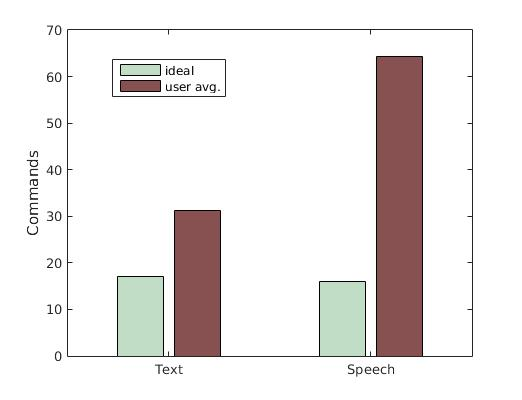
\includegraphics[width=0.8\textwidth]{images/ideal_cmd.jpg}
  \caption{Bladiblala}\label{ideal_cmd}
\end{figure}

Figure \ref{time_cmd} shows the number of commands used over time. As you would expect, the speech version follows the logic of ``the longer time played the more commands used''. However, this is not the case for the text version, where the time played seems irrelevant to the amount of commands used.

\begin{figure}[h!]
  \centering
  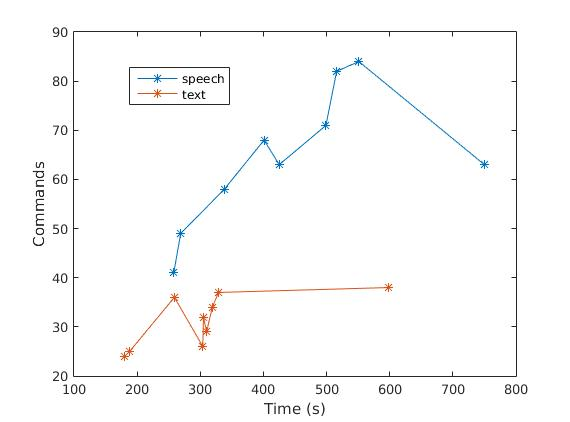
\includegraphics[width=0.8\textwidth]{images/time_cmd.jpg} %width=0.8\textwidth scales the image down to 80 percent of the text-width. Keeps the ratio.
  \caption{Bladiblala}\label{time_cmd}
\end{figure}

\section{Ease of Use}
%OBS!!!! MAYBE DESCRIPTION OF IDEAL SHOULD BE DESCRIBED SOMEWHERE ELSE
When the user played the game, the amount of commands used was recorded. A command is the entire sentence the user inputted into the game. To have something to compare to, the game was played by us to record what would be the minimum amount of commands needed to be used given that the player would have a lot of luck, or the ``ideal'' play-session. The rules used was that when entering a room, ``check room'' were inputted to get the description. No item in the room were checked, just taken or used, unless the puzzle involve looking at an item (such as a note). The result can be seen in figure \ref{ideal_cmd} where amount of commands users used is compared to the ideal for each game. In the text-version there is roughly 2 times the amount of commands as in the ideal, while in the speach-version it is about 4 times.

\subsection{English Confidence} \label{sec:eng_con}
Each user had to rate their spoken and written english between 1-5, where 1 is not good and 5 is fluent. These users were divided into groups and the average amount of commands, time and score were calculated for each group. The result for the amount of commands can be seen in figure \ref{eng_cmd}. 
\begin{figure}[p]
  \centering
  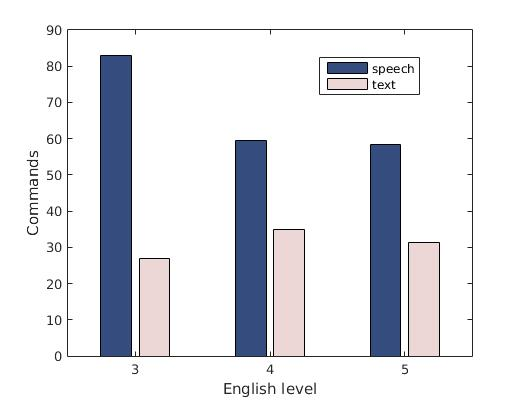
\includegraphics[width=0.8\textwidth]{images/english_cmd.jpg}
  \caption{Bladiblala}\label{eng_cmd}
\end{figure}
The time is put in seconds and is shown in figure \ref{eng_time}.
\begin{figure}[p]
  \centering
  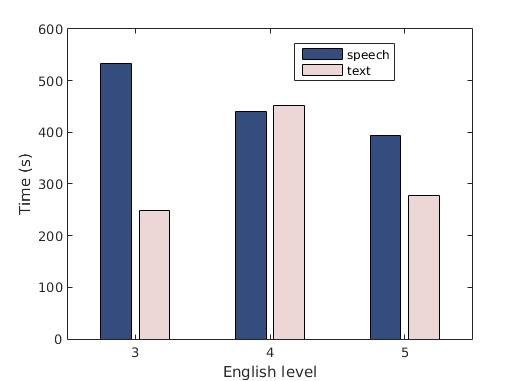
\includegraphics[width=0.8\textwidth]{images/english_time.jpg}
  \caption{Bladiblala}\label{eng_time}
\end{figure}
The score from the System Usability Scale in relation to the english level is displayed in figure \ref{eng_score}.
\begin{figure}[p]
  \centering
  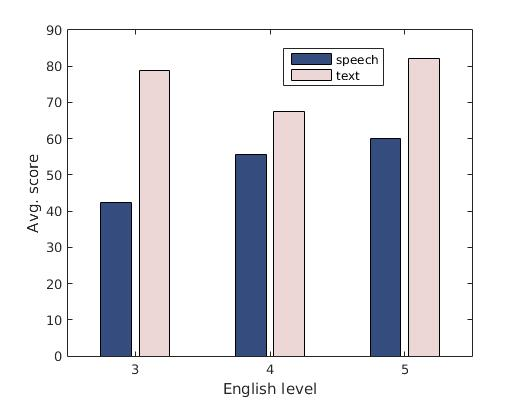
\includegraphics[width=0.8\textwidth]{images/english_score.jpg}
  \caption{Bladiblala}\label{eng_score}
\end{figure}

%\subsection{User Former Experience}

\section{Satisfaction (SUS)}
Figure \ref{sus_table} shows the average answer on each question after they have been converted according to formulae \ref{eq:convert} in section \ref{sec:sus}. 
\begin{figure}[p]
  \centering
  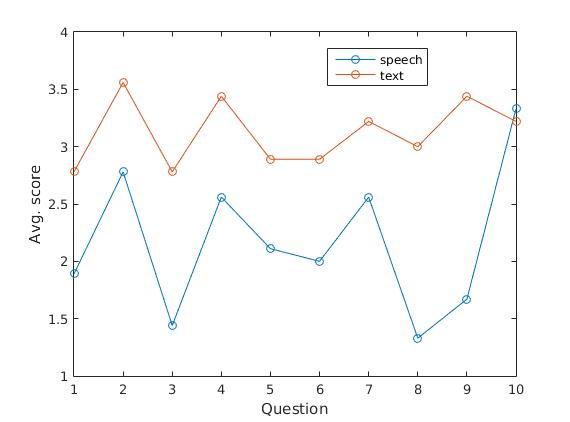
\includegraphics[width=0.8\textwidth]{images/sus.jpg}
  \caption{Bladiblala}\label{sus_table}
\end{figure}

The total average score as calculated in formulae \ref{eq:sum} for each version can be seen in table \ref{tot_score}.
\begin{table}[h!]
  \centering
  \begin{tabular}{ccc}
    \toprule
    Speech &   & Text\\
    \midrule
    54.17 &   & 78.06\\
    \bottomrule
  \end{tabular}
  \caption{Caption for the table.}\label{tot_score}
\end{table}

satisfaction

\chapter{Discussion}
\section{Comparison of Input Methods} %Diskution av resultaten


\section{Sources of Error} %Felkällor


\section{Future Research}

\chapter{Conclusion}
Text is better as input method for NLIs than speech in most cases. It takes less time to perform tasks needed, less tries to get the desired outcome and it has an overall higher usability level. However, if the user is confident in its English competence it will perform tasks with a higher correctness in the speech version. The user will also be more satisfied with it, at a level close to the text version. Given that the user base has English as it's native language, speech is a viable option as input method for NLIs and may be investigated further for that particular usage. For most situations and uses, however, text is much prefered.

\newpage
\addcontentsline{toc}{section}{References}
\bibliographystyle{apalike}
\bibliography{references} % expects file "references.bib"

\appendix
\addappheadtotoc
\chapter{RDF}\label{appA}

\begin{figure}[ht]
\begin{center}
And here is a figure
\caption{\small{Several statements describing the same resource.}}\label{RDF_4}
\end{center}
\end{figure}

that we refer to here: \ref{RDF_4}

\chapter{SUS}\label{appB}
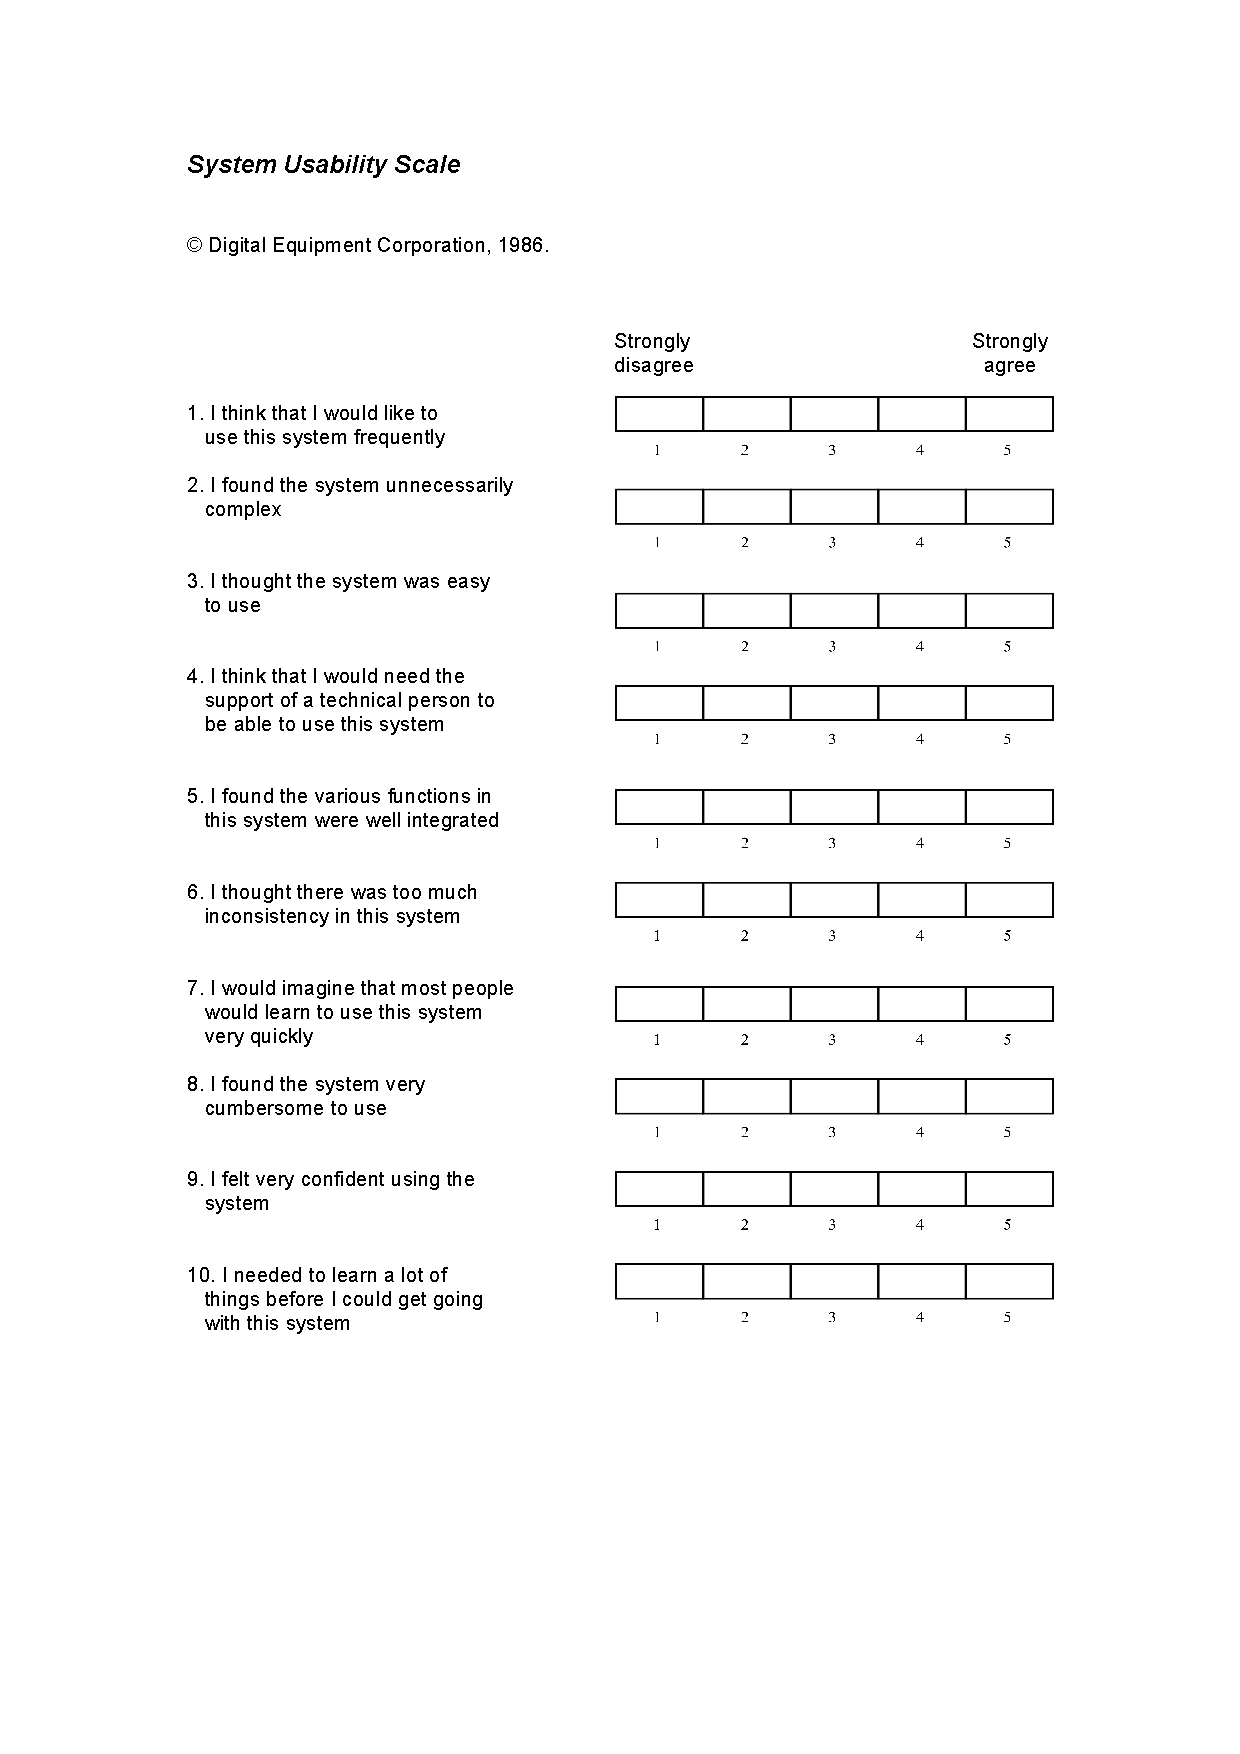
\includegraphics[keepaspectratio, scale = 0.65]{images/suschapt.pdf}\label{Quest}
%\caption{\small{Questions used in the System Usability Scale}}\label{Quest}

\end{document}
